% !TEX program = pdflatex
\documentclass[aspectratio=169,11pt]{beamer}

\usetheme{Madrid}
\usecolortheme{seahorse}
\setbeamertemplate{navigation symbols}{}
\setbeamertemplate{footline}[frame number]

\usepackage[T1]{fontenc}
\usepackage{lmodern}
\usepackage{listings}
\usepackage{booktabs}
\usepackage{tikz}
\usetikzlibrary{arrows.meta,positioning}

\lstset{
  basicstyle=\ttfamily\scriptsize,
  keywordstyle=\color{blue!70!black}\bfseries,
  commentstyle=\color{green!50!black},
  stringstyle=\color{red!60!black},
  breaklines=true,
  showstringspaces=false,
  columns=fullflexible,
  frame=single,
  backgroundcolor=\color{gray!8},
  rulecolor=\color{gray!40},
  xleftmargin=2pt,
  xrightmargin=2pt,
}

\definecolor{beastblue}{RGB}{40,80,140}
\definecolor{beastorange}{RGB}{200,100,20}
\setbeamercolor{frametitle}{fg=beastblue}
\setbeamercolor{title}{fg=beastblue}
\setbeamercolor{structure}{fg=beastblue}

\newcommand{\pkg}[1]{\texttt{\color{beastorange}#1}}
\newcommand{\code}[1]{\texttt{#1}}

\title{BEAST 3 Package Manager}
\subtitle{Design, Storage Models, and Loading Precedence}
\author{BEAST Core Developer Team}
\date{2026}

\begin{document}

\begin{frame}
\titlepage
\end{frame}

% Package manager slides — shared between beast-pkgmgmt-talk.tex and beast3-talk.tex.
% Assumes the preamble defines: \code, \pkg, beastblue, beastorange colours,
% listings, tikz with arrows.meta and positioning.

\begin{frame}{Package System Design Principles}
\begin{enumerate}
\item \textbf{One ModuleLayer per package} --- namespace isolation without losing visibility to the core API. Two packages can bundle different versions of the same library without conflict.

\item \textbf{Same code path for dev and deployment} --- \code{module-info.java} \code{provides} declarations are the single source of truth. A developer in IntelliJ and an end user with an installed ZIP see the same service discovery.

\item \textbf{Graceful degradation} --- modules with unsatisfied dependencies (e.g.\ FX modules on a headless cluster) are silently skipped. Core modules still load.

\item \textbf{First-found wins} --- when the same JPMS module appears in multiple locations (boot layer, installed package, archive), the first one loaded wins. No silent duplicates, no ``reads more than one module'' errors.

\item \textbf{Dual distribution} --- ZIP archives (CBAN) and Maven Central JARs converge on the same ModuleLayer creation path.
\end{enumerate}
\end{frame}

\begin{frame}{Development vs Deployment}
\begin{columns}[T]
\begin{column}{0.48\textwidth}
\textbf{Development (IDE)}
\begin{itemize}
\item All modules in the \textbf{boot layer}
\item IDE resolves module path from Maven
\item Package manager has nothing to do
\item Services discovered via \code{module-info.java}
\item Debug, hot-reload as normal
\end{itemize}
\end{column}
\begin{column}{0.48\textwidth}
\textbf{Deployment (user install)}
\begin{itemize}
\item Only core modules in boot layer
\item External packages loaded into child \textbf{ModuleLayers} at startup
\item Two storage formats coexist
\item Same service discovery mechanism
\end{itemize}
\end{column}
\end{columns}
\end{frame}

\begin{frame}[fragile]{Service Discovery: \code{module-info.java}}
\textbf{Primary mechanism} --- BEAST scans module descriptors at startup:

\begin{lstlisting}[language=Java]
open module my.beast.package {
    requires beast.pkgmgmt;
    requires beast.base;

    provides beast.base.core.BEASTInterface with
        my.beast.package.MyModel,
        my.beast.package.MyOperator;
}
\end{lstlisting}

\begin{itemize}
\item Works in both the boot layer (IDE development) and plugin layers (deployed packages)
\item IntelliJ/Eclipse discover services automatically when both projects are open
\end{itemize}
\end{frame}

\begin{frame}{Service Discovery: \code{version.xml} Fallback}
\begin{itemize}
\item \textbf{Still works} for non-modular JARs
\item JARs without \code{module-info} are treated as automatic modules
\item Services registered from \code{version.xml} as before
\item Useful for gradual migration
\end{itemize}

\vspace{1em}
\begin{block}{Recommendation}
Add \code{module-info.java} when you can --- it's the primary mechanism and gives you compile-time module dependency checking.
\end{block}
\end{frame}

\begin{frame}{Plugin ModuleLayer Isolation}
\begin{center}
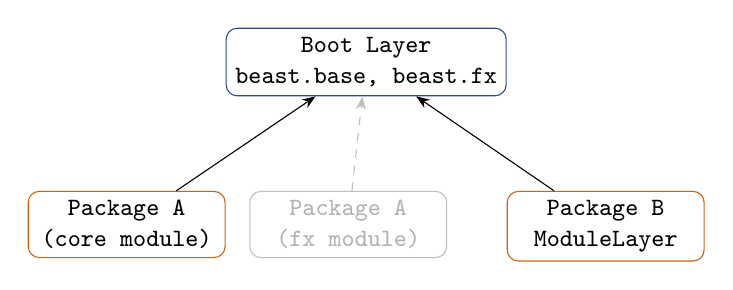
\begin{tikzpicture}[
    box/.style={draw=beastblue, rounded corners, minimum width=2.8cm, minimum height=0.8cm, font=\small\ttfamily, align=center},
    pkg/.style={draw=beastorange, rounded corners, minimum width=2.5cm, minimum height=0.8cm, font=\small\ttfamily, align=center},
    skip/.style={draw=gray!50, rounded corners, minimum width=2.5cm, minimum height=0.8cm, font=\small\ttfamily, align=center, text=gray!60},
    >=Stealth
]
\node[box] (boot) {Boot Layer\\beast.base, beast.fx};
\node[pkg, below left=1.2cm and 0cm of boot] (p1) {Package A\\(core module)};
\node[skip, right=0.3cm of p1] (p1fx) {Package A\\(fx module)};
\node[pkg, below right=1.2cm and 0cm of boot] (p2) {Package B\\ModuleLayer};
\draw[->] (p1) -- (boot);
\draw[->] (p2) -- (boot);
\draw[->, dashed, gray!50] (p1fx) -- (boot);
\end{tikzpicture}
\end{center}

\begin{itemize}
\item Each deployed package gets its \textbf{own ModuleLayer}
\item No classpath conflicts between packages
\item Modules with unsatisfied dependencies (e.g.\ FX modules on a headless cluster) are \textbf{automatically skipped} --- core modules still load
\end{itemize}
\end{frame}

\begin{frame}{Two Storage Models}
Both formats live under \code{\textasciitilde/.beast/2.8/}:

\vspace{0.5em}
\begin{columns}[T]
\begin{column}{0.48\textwidth}
\textbf{ZIP packages} (legacy)
\begin{itemize}
\item One \textbf{subdirectory per package}:\\
  \code{MyPackage/lib/*.jar}\\
  \code{MyPackage/version.xml}
\item Directory structure \emph{is} the index --- any subdirectory with \code{version.xml} is a package
\item No external index needed
\end{itemize}
\end{column}
\begin{column}{0.48\textwidth}
\textbf{Maven packages} (recommended)
\begin{itemize}
\item JARs cached in \code{maven-repo/} --- flat Maven cache with transitive deps mixed together
\item \code{maven-packages.xml} records which coordinates the user installed
\item Index needed because the cache is opaque --- can't tell ``what is a package'' from directory structure alone
\end{itemize}
\end{column}
\end{columns}

\vspace{0.5em}
\begin{block}{Why two models?}
ZIP packages are self-describing (directory = package). Maven packages need an explicit index because the local cache holds transitive dependencies alongside the package itself.
\end{block}
\end{frame}

\begin{frame}{Package Loading Precedence}
\textbf{\code{PackageManager.loadExternalJars()}} runs when BEAST starts:

\vspace{0.5em}
\begin{enumerate}
\item \textbf{Load Maven packages} --- resolve coordinates from \code{maven-packages.xml}, create a ModuleLayer per package. Maven is the recommended format, so these take precedence.
\item \textbf{Scan package directories} --- find installed ZIP packages in\\
  \code{\textasciitilde/.beast/2.8/} (or \code{BEAST\_PACKAGE\_PATH})
\item \textbf{Create ModuleLayer per ZIP package:}
  \begin{itemize}
  \item Discover JPMS modules from the package's JARs
  \item Exclude modules already in boot layer or Maven layers (no duplicates)
  \item Filter out modules whose \code{requires} can't be satisfied
  \item \code{resolveAndBind()} on the remaining modules
  \end{itemize}
\item \textbf{Register with \code{BEASTClassLoader}} --- services from both \code{module-info.java} and \code{version.xml} merged into registry
\end{enumerate}

\vspace{0.3em}
\textbf{Precedence:} boot layer $\to$ Maven $\to$ ZIP.  If the same module exists in both formats, the Maven version wins.
\end{frame}

\begin{frame}{Maven Central Distribution}
\textbf{New:} packages can be published as plain Maven Central JARs.

\vspace{0.5em}
\begin{itemize}
\item Users install via BEAUti: \textbf{Install from Maven} button
\item Or CLI: \code{packagemanager -maven groupId:artifactId:version}
\item Resolution via Apache Maven Resolver
\item JARs cached in \code{\textasciitilde/.beast/2.8/maven-repo/}
\item Tracked in \code{maven-packages.xml}
\end{itemize}

\vspace{0.5em}
\begin{itemize}
\item Custom repos: \code{packagemanager -addMavenRepository <url>}
\item ZIP packages still work alongside Maven packages
\end{itemize}
\end{frame}

\begin{frame}{\code{beast-package-skeleton}}
Ready-to-copy template project on GitHub:

\vspace{0.5em}
\begin{itemize}
\item Maven \code{pom.xml} with BEAST 3 dependencies
\item \code{module-info.java} with \code{provides} declarations
\item Example \code{ScalarDistribution}, operator, and tests
\item BEAST XML using the strongly-typed spec API
\item Maven Central release profile (source, javadoc, GPG, publishing plugin)
\item \code{version.xml} JAR embedding
\end{itemize}

\vspace{1em}
\begin{exampleblock}{}
Start here: \url{https://github.com/CompEvol/beast-package-skeleton}
\end{exampleblock}
\end{frame}


\end{document}
